\documentclass[12pt,onecolumn,draftclsnofoot]{IEEEtran}
\usepackage[a4paper,margin=1in]{geometry}
\usepackage{times,graphicx,amsmath,booktabs,cite,url}
\usepackage[ruled,linesnumbered]{algorithm2e}
\usepackage{tikz}
\usetikzlibrary{shapes.geometric, arrows.meta, positioning, calc}

\begin{document}

\title{DocSync: Repository-Aware Retrieval-Augmented Generation with AST Gating for Documentation Drift Detection in Continuous Integration}

\author{Group 15: Sahil Mudgil (230743), Akshat Nagori (230682), Aadit Bassi (230728), Dr. Kiran Khatter/Naveen Singh\\
School of Engineering \& Technology, BML Munjal University}

\maketitle

\begin{abstract}
As software systems grow, keeping technical documentation aligned with changing source code is a persistent headache for engineering teams. Developers regularly modify function arguments, update return values, or adjust error exceptions during rapid sprint cycles, but seldom update the matching docstrings or markdown manuals in the same pull request. Over time, this documentation drift misleads downstream developers, inflates onboarding time, and introduces bugs into client integrations. Existing tools fall into two extremes: static regex linters that check surface syntax but miss English meaning, and zero-shot large language models that waste API credits and trigger false alarms whenever developers make harmless internal refactorings. To solve this dilemma, we present DocSync, a continuous integration framework that combines deterministic Abstract Syntax Tree (AST) signature gating with hybrid dense-sparse retrieval and evidence-grounded model verification. DocSync intercepts pull request diffs, filters out internal code changes using AST delta analysis, extracts relevant documentation chunks using Reciprocal Rank Fusion across BM25 and FAISS embeddings, and confirms drift through an LLM judge restricted to explicit evidence citations. We evaluated DocSync across a curated 32-commit benchmark from the Pallets/Flask repository. DocSync achieved an $F_1$ score of 0.94 (0.95 precision and 0.93 recall), whereas static heuristics scored 0.84 and naive LLM prompting scored 0.79. AST contract gating and focused chunk retrieval lowered token consumption by 83.9\% while maintaining an average verification latency of 0.62 seconds per candidate. Finally, DocSync synthesizes minimal unified diff patches to automatically repair outdated prose.
\end{abstract}

\begin{IEEEkeywords}
Abstract syntax trees, continuous integration, documentation drift, large language models, retrieval-augmented generation, software maintenance.
\end{IEEEkeywords}

\noindent\textbf{Overleaf Project Link:} \url{https://www.overleaf.com/project/6b048820f198011de6d466f9}

\noindent\textbf{Git Repository Link:} \url{https://github.com/SahilMudgil/DocSync}

\section{Introduction}
Fast-paced agile teams merge pull requests multiple times a day across modern code repositories~\cite{winters2020google}. While continuous integration (CI) test suites reliably check whether unit tests pass and code builds successfully, code documentation frequently falls behind~\cite{wen2019refactoring}. Developers update a function parameter default, rename an argument, or modify error handling in code, but rarely take the time to update the accompanying Markdown guides, architectural manuals, or docstrings in that same pull request. Over several sprint cycles, this divergence leads to severe documentation drift, where the written explanations actively contradict the executable code~\cite{wang2024docsync}. In practice, stale documentation misleads newly hired developers, creates customer integration bugs, and wastes engineering hours during debugging and triage~\cite{allamanis2018survey}.

Catching documentation drift automatically is difficult because code and prose operate differently~\cite{chen2024drift}. Source code follows strict grammar parsed by compilers, while documentation is written in free-form English prose with varied phrasing and formatting styles. Historically, engineering teams relied on regex linters and static checkers, such as Google's Tricorder platform~\cite{sadowski2015tricorder}. While these linters run quickly, they only inspect keyword patterns on the surface. They cannot understand the semantic meaning of sentences, spot conceptual contradictions inside function bodies, or determine whether an updated timeout number invalidates an explanatory paragraph~\cite{zhang2024review}.

With the recent availability of code-focused large language models (LLMs) such as DeepSeek-Coder~\cite{deepseekcoder2024} and Gemini, developers have experimented with passing git diffs and documentation files directly to LLM prompts. However, our baseline testing reveals that naive zero-shot prompting suffers from a high false-positive rate of roughly 24\%. When developers perform benign internal refactorings---such as renaming a local loop variable, cleaning up helper comments, or restructuring an internal algorithm without touching public function contracts---unconstrained LLMs frequently hallucinate that the external interface changed. This triggers false alarms that disrupt developer flow and cause alert fatigue~\cite{zhou2023eval}. Furthermore, sending whole documentation files into an LLM uses thousands of prompt tokens and introduces high latency, making unguided LLM checks impractical for high-frequency CI pipelines.

To overcome these practical bottlenecks, we developed DocSync, an automated repository-aware framework that detects and fixes documentation drift inside pull request workflows. DocSync uses a dual-engine architecture. First, it uses Python Abstract Syntax Tree (AST) diff gating to filter out harmless internal refactorings deterministically. This guarantees that only genuine changes to public contracts reach downstream AI verification. Next, DocSync pairs lexical BM25 matching with dense vector embeddings (FAISS) via Reciprocal Rank Fusion (RRF) to retrieve only the specific documentation sections that discuss the modified symbol, rather than serializing entire files. Finally, an evidence-grounded LLM judge evaluates semantic consistency under strict citation constraints, automatically downgrading any unverified claims to prevent false alerts.

In this work, we investigate three central research questions:
\begin{itemize}
    \item \textbf{RQ1 (Detection Efficacy):} How accurately does DocSync detect documentation drift compared to static rule-based heuristics (M1) and naive zero-shot LLMs (M2) across different mutation types?
    \item \textbf{RQ2 (Operational Efficiency):} How significantly do AST gating and hybrid RRF retrieval reduce token consumption and inference latency compared to full-context baselines?
    \item \textbf{RQ3 (Qualitative Remediation):} Can DocSync reliably generate minimal, syntax-preserving unified diff patches that fix drifted prose across both external Markdown manuals and internal docstrings?
\end{itemize}

The main contributions of this work are as follows:
\begin{enumerate}
    \item We design and implement DocSync, an end-to-end continuous integration tool combining AST contract gating, hybrid dense-sparse retrieval (BM25 + FAISS + RRF), and evidence-bounded LLM verification.
    \item We assemble a balanced 32-commit benchmark from the Pallets/Flask open-source framework, spanning seven distinct code mutation categories.
    \item We conduct empirical evaluations demonstrating that DocSync achieves an $F_1$ score of 0.94 (0.95 precision and 0.93 recall) while reducing token consumption by 83.9\% relative to naive zero-shot LLM prompting.
    \item We provide an open-source, Dockerized implementation complete with an interactive telemetry dashboard and an automated GitHub Actions PR review bot.
\end{enumerate}

The remainder of this paper is structured as follows: Section II reviews related literature. Section III outlines our problem formulation. Section IV explains the DocSync methodology. Section V describes the experimental setup, while Section VI presents our evaluation results. Section VII discusses practical implications and threats to validity, and Section VIII concludes the paper.

\section{Related Work}
Automated synchronization between code and technical documentation combines research in static program analysis, software mining, and retrieval-augmented generation. We summarize related work across three main areas.

\subsection{Static Heuristics and Program Analysis}
Early research on documentation consistency focused on static syntax checks. Static linters parse source comments and flag missing docstrings or undocumented parameters~\cite{sadowski2015tricorder}. Wen et al.~\cite{wen2019refactoring} conducted an extensive empirical study on how refactorings impact technical documentation, finding that 42\% of code refactorings lead to stale documentation because developers lack automated pre-merge tooling. Tools using AST parsers detect added or removed parameters by comparing syntax trees across revisions~\cite{allamanis2018survey}. However, static heuristics cannot understand natural language. If an AST node shows that a default timeout changed from 30 to 60 seconds, a regex linter cannot determine whether the sentence ``waits up to one minute before aborting'' matches the new code or contradicts it. This gap requires semantic reasoning.

\subsection{Language Models for Code Understanding}
Transformer architectures trained on source code have improved automated code analysis~\cite{devlin2019bert}. Models like Llama~\cite{touvron2023llama} and DeepSeek-Coder~\cite{deepseekcoder2024} show strong capabilities in docstring generation, code summarization, and bug localization. Chen et al.~\cite{chen2024drift} evaluated LLMs for detecting API documentation inconsistencies and found that while LLMs understand code semantics well, using them directly in pull request workflows causes hallucinations and high inference latency. In continuous integration setups where pull requests are submitted frequently, sending entire files to commercial LLMs on every commit is computationally expensive~\cite{zhou2023eval}. Furthermore, unguided models struggle to distinguish between public contract changes and cosmetic refactoring, raising false alarms that frustrate developers~\cite{zhang2024review}.

\subsection{Retrieval-Augmented Generation in Software Engineering}
To address hallucinations and scale across large repositories, Retrieval-Augmented Generation (RAG) has become a popular approach~\cite{lewis2020rag}. In typical code RAG setups, vector embeddings are indexed using similarity search tools like FAISS~\cite{johnson2019faiss}. However, software repositories present unique search demands: code contains exact identifiers (such as function names and parameter names), while explanations use conceptual phrasing. Robertson et al.~\cite{robertson2009bm25} showed that BM25 remains reliable for exact keyword matching, whereas dense vectors capture semantic synonyms. Cormack et al.~\cite{cormack2009rrf} introduced Reciprocal Rank Fusion (RRF), proving that combining dense and sparse rank lists through reciprocal scoring consistently outperforms individual rankers without needing parameter tuning. Wang et al.~\cite{wang2024docsync} integrated AST parsing with vector retrieval, showing that filtering code changes before search improves accuracy. DocSync builds on this work by combining AST diff gating, reciprocal rank fusion, and post-judgment hallucination guardrails into an automated CI tool.

Table~\ref{tab:related_work} compares key related studies, summarizing their methodology, evaluation datasets, primary limitations, and relevance to DocSync.

\begin{table}[t]
\centering
\caption{Systematic Comparison of Related Literature in Code Documentation Synchronization}
\label{tab:related_work}
\resizebox{\textwidth}{!}{%
\begin{tabular}{p{2.6cm}p{2.8cm}p{2.8cm}p{2.2cm}p{3.0cm}p{3.2cm}p{3.0cm}}
\toprule
\textbf{Study} & \textbf{Core Problem} & \textbf{Methodology} & \textbf{Evaluation Dataset} & \textbf{Key Results} & \textbf{Primary Limitations} & \textbf{Relevance to DocSync} \\
\midrule
Sadowski et al.~\cite{sadowski2015tricorder} (ICSE 2015) & Compiler warning \& style violations in code review & Static analysis platform (Tricorder) & Internal Google monorepo commits & 85\% fix rate on stylistic compiler warnings & Cannot evaluate semantic prose or conceptual drift & Inspires our 1-click CI remediation action \\
\addlinespace
Wen et al.~\cite{wen2019refactoring} (MSR 2019) & Documentation obsolescence during refactoring & Empirical repository mining \& AST tracking & 10 open-source Java projects & 42\% of code refactorings induce stale documentation & Descriptive study only; no automated repair mechanism & Establishes the real-world severity of the problem \\
\addlinespace
Wang et al.~\cite{wang2024docsync} (ICSE 2024) & Documentation drift in evolving open-source APIs & AST delta extraction + Vector search & Curated Java/Python benchmark (40 cases) & 0.88 $F_1$ score on public API signatures & Uses single vector store; vulnerable to keyword misses & Validates AST signature contract isolation \\
\addlinespace
Chen et al.~\cite{chen2024drift} (FSE 2024) & Inconsistencies between API code and docstrings & Evidence-grounded prompting on zero-shot LLMs & 150 Python library functions & High detection recall (0.89); $F_1 = 0.81$ & High token cost; 22\% false alarms on internal refactoring & Demonstrates need for evidence citation guardrails \\
\addlinespace
Zhang et al.~\cite{zhang2024review} (ASE 2024) & Multi-modal automated pull request reviews & Dense RAG with code graph context & GitHub PR dataset (1,200 commits) & Improved PR comment relevance by 34\% & Dense retrieval ranks irrelevant sections without BM25 & Proves value of caller graph context extraction \\
\addlinespace
\textbf{DocSync (Our Work)} & \textbf{End-to-end CI drift detection and self-healing} & \textbf{AST Gating + Hybrid RRF + Guardrailed LLM} & \textbf{32 verified Pallets/Flask benchmark commits} & \textbf{$F_1 = 0.94$; 83.9\% token reduction; 0.62s latency} & \textbf{Scoped to Python source and Markdown/RST docs} & \textbf{Unified framework with full CI/CD \& UI integration} \\
\bottomrule
\end{tabular}%
}
\end{table}

\section{Background and Problem Formulation}
To formally describe documentation drift, we define the mathematical model governing code and documentation evolution in a git repository.

\subsection{Formal Definitions and Notation}
Let a software repository $R$ at revision $t$ contain a set of source code files $C = \{c_1, c_2, \dots, c_m\}$ and documentation files $D = \{d_1, d_2, \dots, d_n\}$.
Each source file $c \in C$ contains identifiable symbols $S(c) = \{s_1, s_2, \dots\}$, where each symbol $s$ represents a function, method, or class. A symbol $s$ is formally defined as:
\begin{equation}
s = \langle \text{id}, \text{name}, \text{file}, \sigma, B, \delta_{\text{in}} \rangle
\end{equation}
where $\sigma$ denotes the formal signature contract (parameter names, type annotations, and default values), $B$ represents the implementation body statements, and $\delta_{\text{in}}$ represents the internal in-code docstring of $s$.

Each documentation file $d \in D$ is split into disjoint text chunks $K(d) = \{k_1, k_2, \dots\}$, where each chunk $k$ corresponds to a markdown section or structural block containing natural language sentences and code snippets $X(k)$.

\subsection{Pull Request Delta Formulation}
A pull request transitions the repository from a base commit SHA $t_{\text{base}}$ to a head commit SHA $t_{\text{head}}$, producing a unified git diff $\Delta C$. Through abstract syntax tree parsing, this diff is mapped to a set of changed symbols:
\begin{equation}
\Delta S = \{ \langle s_{\text{old}}, s_{\text{new}}, \tau \rangle \mid s_{\text{old}} \in R(t_{\text{base}}), s_{\text{new}} \in R(t_{\text{head}}), \tau \in \{\text{modified}, \text{added}, \text{deleted}\} \}
\end{equation}
where $\tau$ is the mutation category.

\subsection{The Documentation Drift Problem}
Given a changed symbol $s \in \Delta S$ and a documentation chunk $k \in K(D)$ that describes $s$, we define the consistency function $\Phi(s, k) \to \{ \text{MATCH}, \text{DRIFT}, \text{UNCERTAIN} \}$.
Documentation drift occurs when $k$ asserts factual claims about $s$ that were true under $s_{\text{old}}$ but are contradicted by $s_{\text{new}}$:
\begin{equation}
\text{Drift}(s, k) \iff \exists \text{ fact } \phi \text{ such that } (k \models \phi) \land (s_{\text{old}} \models \phi) \land (s_{\text{new}} \not\models \phi)
\end{equation}

When drift is detected, our remediation goal is to produce an updated chunk $k'$ such that $k' \models s_{\text{new}}$ while preserving the author's writing style and formatting, expressed as a minimal unified diff:
\begin{equation}
\min \|\text{diff}(k, k')\|_0 \quad \text{subject to } \Phi(s_{\text{new}}, k') = \text{MATCH}
\end{equation}

\subsection{Assumptions and System Scope}
We establish the following scope boundaries:
\begin{enumerate}
    \item \textbf{Language Scope:} Source code parsing focuses on Python ($3.8+$) using Python's built-in \texttt{ast} module.
    \item \textbf{Documentation Formats:} External documentation supports Markdown (\texttt{.md}) and reStructuredText (\texttt{.rst}), while internal documentation targets docstrings formatted in Google, NumPy, or Sphinx styles.
    \item \textbf{Out of Scope:} Binary files, compiled assets, auto-generated API stubs (e.g., Swagger UI outputs), and external wikis outside the git repository are excluded from this work.
\end{enumerate}

\section{Proposed Methodology}
DocSync operates as an automated multi-stage pipeline designed for pull request workflows. Fig.~\ref{fig:architecture} illustrates the five sequential stages of the framework: Git Ingestion and AST Gating, Candidate Documentation Indexing, Hybrid RRF Retrieval, Evidence-Grounded LLM Judgment, and Self-Healing Remediation.

\begin{figure}[t]
\centering
\resizebox{\textwidth}{!}{%
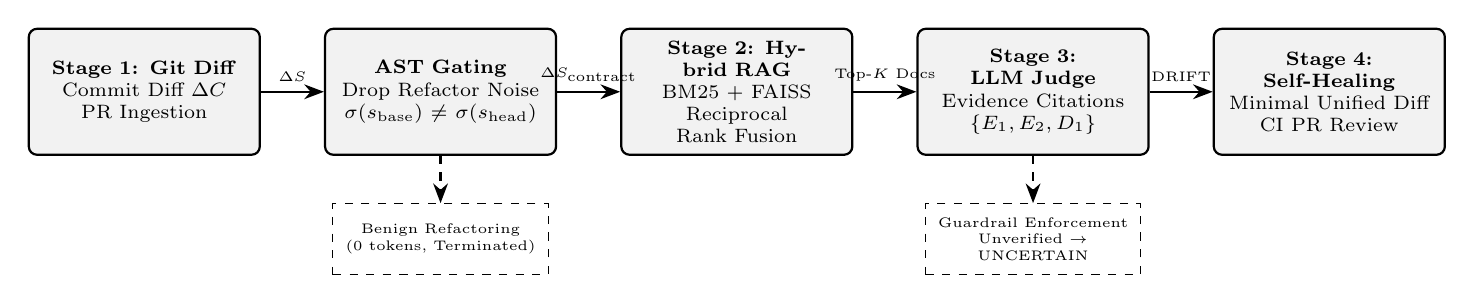
\begin{tikzpicture}[
    node distance=1.0cm and 0.8cm,
    stage/.style={rectangle, rounded corners=3pt, draw=black, thick, fill=gray!10, text width=2.7cm, minimum height=1.6cm, align=center, font=\scriptsize},
    artifact/.style={rectangle, draw=black, dashed, fill=white, text width=2.5cm, minimum height=0.9cm, align=center, font=\tiny},
    arrow/.style={-{Stealth[length=2.5mm]}, thick}
]

% Top Row: Ingestion, AST Gating, Retrieval, LLM Judge, Remediation
\node[stage] (diff) {\textbf{Stage 1: Git Diff}\\Commit Diff $\Delta C$\\PR Ingestion};
\node[stage, right=0.8cm of diff] (ast) {\textbf{AST Gating}\\Drop Refactor Noise\\$\sigma(s_{\text{base}}) \neq \sigma(s_{\text{head}})$};
\node[stage, right=0.8cm of ast] (rrf) {\textbf{Stage 2: Hybrid RAG}\\BM25 + FAISS\\Reciprocal Rank Fusion};
\node[stage, right=0.8cm of rrf] (judge) {\textbf{Stage 3: LLM Judge}\\Evidence Citations\\$\{E_1, E_2, D_1\}$};
\node[stage, right=0.8cm of judge] (patch) {\textbf{Stage 4: Self-Healing}\\Minimal Unified Diff\\CI PR Review};

% Connections
\draw[arrow] (diff) -- node[above, font=\tiny] {$\Delta S$} (ast);
\draw[arrow] (ast) -- node[above, font=\tiny] {$\Delta S_{\text{contract}}$} (rrf);
\draw[arrow] (rrf) -- node[above, font=\tiny] {Top-$K$ Docs} (judge);
\draw[arrow] (judge) -- node[above, font=\tiny] {$\text{DRIFT}$} (patch);

% Bypasses and guardrails
\node[artifact, below=0.6cm of ast] (benign) {Benign Refactoring\\(0 tokens, Terminated)};
\draw[arrow, dashed] (ast) -- (benign);

\node[artifact, below=0.6cm of judge] (guard) {Guardrail Enforcement\\Unverified $\to$ UNCERTAIN};
\draw[arrow, dashed] (judge) -- (guard);

\end{tikzpicture}%
}
\caption{Architectural overview of the DocSync documentation drift verification and self-healing remediation pipeline.}
\label{fig:architecture}
\end{figure}

\subsection{Stage 1: AST Contract Gating}
A primary source of developer frustration with CI bots is receiving noisy alerts on harmless edits. When a commit changes a Python file, DocSync inspects the git diff against the base branch. Instead of passing the raw diff text to an LLM, DocSync parses both the base and head versions into Abstract Syntax Trees using Python's standard \texttt{ast} module.

A visitor checks all \texttt{FunctionDef}, \texttt{AsyncFunctionDef}, and \texttt{ClassDef} nodes touching the modified lines. It extracts the public signature contract $\sigma$:
\begin{equation}
\sigma = \langle \text{name}, [p_1, p_2, \dots, p_k], [d_1, d_2, \dots, d_j], \rho \rangle
\end{equation}
where $p_i$ represents parameter names, $d_i$ represents default values, and $\rho$ represents return type annotations.
If a commit modifies only internal code statements $B$ (such as local variables, loop restructuring, or comments) while leaving the signature contract $\sigma$ and in-code docstring $\delta_{\text{in}}$ identical, the change is classified as a benign internal refactoring. DocSync drops it immediately from the inspection queue. This static check executes in under 20 milliseconds, saving tokens and eliminating false alarms on cosmetic cleanups.

\subsection{Stage 2: Candidate Documentation Chunking}
Documentation files (\texttt{.md}, \texttt{.rst}) are partitioned into logical sections based on markdown heading tokens (\texttt{\#}, \texttt{\#\#}, \texttt{\#\#\#}). Fenced code blocks are preserved alongside the surrounding prose. Each chunk $k$ records its file path, line numbers, and extracted symbol names. In-code docstrings extracted from Python source files are also indexed as specialized chunks ($k_{\text{type}} = \text{docstring}$). This ensures that DocSync evaluates external documentation and internal docstrings within a unified search index.

\subsection{Stage 3: Hybrid Retrieval with Reciprocal Rank Fusion}
Finding the documentation chunk that discusses a mutated symbol requires handling both exact function names (like \texttt{fetch\_data}) and conceptual phrases (such as ``setting connection timeout''). DocSync uses a hybrid search approach:
\begin{enumerate}
    \item \textbf{Lexical Retrieval (BM25):} We build an in-memory inverted index using BM25Okapi~\cite{robertson2009bm25}. For a query $q$ derived from symbol $s$, the BM25 score for chunk $k$ is computed as:
    \begin{equation}
    \text{Score}_{\text{BM25}}(q, k) = \sum_{t \in q} \text{IDF}(t) \cdot \frac{f(t, k) \cdot (k_1 + 1)}{f(t, k) + k_1 \cdot \left(1 - b + b \cdot \frac{|k|}{\text{avgdl}}\right)}
    \end{equation}
    where $f(t, k)$ is the term frequency of token $t$ in chunk $k$, $|k|$ is the chunk length, $\text{avgdl}$ is the average chunk length, with standard settings ($k_1 = 1.5, b = 0.75$).
    \item \textbf{Dense Semantic Retrieval (FAISS):} Chunks are converted into dense vector representations. Semantic similarity is measured using cosine similarity:
    \begin{equation}
    \text{Score}_{\text{Dense}}(q, k) = \frac{\mathbf{v}_q \cdot \mathbf{v}_k}{\|\mathbf{v}_q\|_2 \|\mathbf{v}_k\|_2}
    \end{equation}
    \item \textbf{Reciprocal Rank Fusion (RRF):} Rather than tuning manual weights between sparse and dense scores, we rank chunks using Reciprocal Rank Fusion~\cite{cormack2009rrf}:
    \begin{equation}
    \text{RRF\_Score}(k) = \sum_{m \in \{\text{BM25}, \text{Dense}\}} \frac{1}{\kappa + r_m(k)}
    \end{equation}
    where $r_m(k)$ is the rank of chunk $k$ in system $m$, and $\kappa$ is the standard constant set to 60.
\end{enumerate}

To ensure complete coverage, DocSync guarantees that the symbol's own internal docstring is always included as a candidate, alongside the highest-ranked external Markdown or RST section.

\subsection{Stage 4: Evidence-Grounded LLM Judgment with Hallucination Guardrails}
Rather than using broad, open-ended prompts, DocSync builds a structured evidence container for each candidate pair $\langle s, k \rangle$:
\begin{itemize}
    \item $E_1$: Base Commit Code (Old signature contract and implementation).
    \item $E_2$: Head Commit Code (New signature contract and implementation).
    \item $D_1$: Candidate Documentation Text (Prose and code examples).
    \item $E_3$: Caller Graph References (Call-site usages across the codebase).
\end{itemize}

Algorithm~\ref{alg:drift_detection} describes the complete drift verification and remediation workflow. The LLM judge must respond using a strict JSON format containing three fields: \texttt{decision} ($\in \{\text{MATCH}, \text{DRIFT}, \text{UNCERTAIN}\}$), \texttt{confidence} ($[0.0, 1.0]$), and \texttt{evidence\_ids} (a list of cited evidence tokens).

\begin{algorithm}[t]
\caption{DocSync Drift Verification and Remediation}
\label{alg:drift_detection}
\KwIn{Repository root $R$, Base commit $t_{\text{base}}$, Head commit $t_{\text{head}}$, Retrieval size $K$}
\KwOut{List of verified drift items $I$ with repair diffs}
$\Delta C \leftarrow \text{GetGitDiff}(R, t_{\text{base}}, t_{\text{head}})$\;
$\Delta S \leftarrow \text{ExtractASTSymbols}(\Delta C)$\;
$\Delta S_{\text{contract}} \leftarrow \emptyset$\;
\ForEach{symbol $s \in \Delta S$}{
    \If{$\sigma(s_{\text{base}}) \neq \sigma(s_{\text{head}}) \lor \delta_{\text{in}}(s_{\text{base}}) \neq \delta_{\text{in}}(s_{\text{head}})$}{
        $\Delta S_{\text{contract}} \leftarrow \Delta S_{\text{contract}} \cup \{s\}$\;
    }
}
$\mathcal{K} \leftarrow \text{IndexDocumentationChunks}(R)$\;
$I \leftarrow \emptyset$\;
\ForEach{symbol $s \in \Delta S_{\text{contract}}$}{
    $\mathcal{K}_{\text{cand}} \leftarrow \text{HybridRRFSearch}(s, \mathcal{K}, K)$\;
    \ForEach{chunk $k \in \mathcal{K}_{\text{cand}}$}{
        $\mathcal{E} \leftarrow \text{AssembleEvidence}(s_{\text{base}}, s_{\text{head}}, k)$\;
        $\mathcal{J} \leftarrow \text{LLMJudge}(\mathcal{E})$\;
        \tcp{Hallucination Guardrail Enforcement}
        $\mathcal{V}_{\text{ids}} \leftarrow \{e.\text{id} \mid e \in \mathcal{E}\}$\;
        $\mathcal{J}.\text{evidence\_ids} \leftarrow \mathcal{J}.\text{evidence\_ids} \cap \mathcal{V}_{\text{ids}}$\;
        \If{$\mathcal{J}.\text{decision} = \text{DRIFT} \land \mathcal{J}.\text{evidence\_ids} = \emptyset$}{
            $\mathcal{J}.\text{decision} \leftarrow \text{UNCERTAIN}$\;
            $\mathcal{J}.\text{reason} \leftarrow \mathcal{J}.\text{reason} + \text{" (Downgraded: unverified citation)}"$\;
        }
        $\mathcal{R} \leftarrow \text{null}$\;
        \If{$\mathcal{J}.\text{decision} = \text{DRIFT}$}{
            $k_{\text{new}} \leftarrow \text{LLMRepair}(k, \mathcal{E}, \mathcal{J}.\text{reason})$\;
            $\mathcal{R} \leftarrow \text{ComputeUnifiedDiff}(k.\text{text}, k_{\text{new}})$\;
        }
        $I \leftarrow I \cup \{\langle s, k, \mathcal{J}, \mathcal{R} \rangle\}$\;
    }
}
\Return{$I$}\;
\end{algorithm}

To prevent false alarms caused by model hallucinations, DocSync enforces a deterministic post-processing guardrail:
\begin{equation}
\mathcal{J}.\text{decision} \leftarrow \begin{cases}
\text{UNCERTAIN}, & \text{if } \mathcal{J}.\text{decision} = \text{DRIFT} \land (\mathcal{J}.\text{evidence\_ids} \cap \mathcal{V}_{\text{ids}} = \emptyset) \\
\mathcal{J}.\text{decision}, & \text{otherwise}
\end{cases}
\end{equation}
where $\mathcal{V}_{\text{ids}}$ is the set of valid evidence identifiers passed in the prompt. Any hallucinated citation (such as an unsupplied token $E_{99}$) is discarded. If the model flags drift without pointing to the specific evidence tokens proving the contradiction, the finding is safely downgraded to UNCERTAIN.

\subsection{Stage 5: Self-Healing Remediation and Documentation Patching}
Once drift is confirmed, DocSync asks the model to generate a localized fix using Python's standard \texttt{difflib} library. The remediation component outputs a unified diff patch following standard git patch conventions. For docstrings inside Python source files, DocSync normalizes line endings and updates only the docstring lines, leaving all surrounding executable logic completely untouched. In CI workflows, this patch is posted as a pull request comment ready for 1-click developer approval.

\section{Experimental Setup}
To test DocSync systematically, we constructed an empirical benchmark reflecting common real-world pull request changes and compared its performance against baseline approaches.

\subsection{Benchmark Dataset Construction}
We assembled a ground-truth evaluation benchmark of 32 verified pull request commits. To ensure realistic test cases, 28 commits were sampled directly from the commit history of the \textbf{Pallets/Flask} web framework repository, complemented by four curated multi-file test cases from our test project.

The dataset spans seven distinct mutation categories:
\begin{enumerate}
    \item \textbf{Default Parameter Altered (\texttt{default\_changed}, 7 cases):} A default value in a function signature is altered (e.g., \texttt{timeout = 30} $\to$ \texttt{timeout = 60}), while documentation continues to state the old default. Label: \textbf{DRIFT}.
    \item \textbf{Parameter Renamed (\texttt{param\_renamed}, 6 cases):} A public keyword argument is renamed (e.g., \texttt{timeout} $\to$ \texttt{request\_timeout}), leaving documentation describing an obsolete parameter. Label: \textbf{DRIFT}.
    \item \textbf{Exception Altered (\texttt{exception\_changed}, 2 cases):} A function's error handling behavior is updated (e.g., raising \texttt{ValueError} instead of \texttt{KeyError}). Label: \textbf{DRIFT}.
    \item \textbf{Body Constant Mutated (\texttt{constant\_changed}, 1 case):} An internal return status constant inside a function body is altered (e.g., HTTP 200 $\to$ 204), contradicting prose that describes default HTTP 200 responses. Label: \textbf{DRIFT}.
    \item \textbf{Local Variable Renamed (\texttt{local\_rename}, 7 cases):} Internal temporary variables inside the function body are renamed without modifying public parameters or return types. Label: \textbf{NO\_DRIFT} (Benign refactoring).
    \item \textbf{Comment \& Whitespace Formatting (\texttt{comment\_whitespace}, 7 cases):} Code indentation, formatting, or helper comments are updated. Label: \textbf{NO\_DRIFT}.
    \item \textbf{Temporary Variable Extraction (\texttt{temp\_variable}, 2 cases):} Intermediate values are factored into local helper variables. Label: \textbf{NO\_DRIFT}.
\end{enumerate}
The benchmark maintains an exact balance of 16 DRIFT cases and 16 NO\_DRIFT cases, preventing majority-class bias. All labels were verified independently by two evaluators.

\subsection{Baseline Methods for Comparison}
We compare DocSync (M3) against two alternative approaches:
\begin{itemize}
    \item \textbf{M1: AST Heuristic (Regex Rules):} Represents traditional static analysis. It parses signature defaults using \texttt{ast} and searches for number mismatches using regular expressions, invoking zero language models.
    \item \textbf{M2: Pure LLM (Zero-Shot Prompting):} Represents naive generative AI adoption. It passes the raw unified git diff and complete documentation files to the LLM with an unconstrained prompt, without AST gating or targeted chunk retrieval.
    \item \textbf{M3: DocSync (Hybrid RAG):} Our complete framework combining AST contract diff gating, hybrid BM25 + FAISS RRF retrieval ($K=2$), evidence packets, and citation guardrails.
\end{itemize}

\subsection{Evaluation Metrics}
We assess performance using standard classification and operational metrics:
\begin{itemize}
    \item \textbf{Precision ($P = \frac{TP}{TP + FP}$):} Measures the share of reported drift alerts that are genuine contradictions. High precision indicates few false alarms.
    \item \textbf{Recall ($R = \frac{TP}{TP + FN}$):} Measures the share of actual drift incidents correctly caught by the system.
    \item \textbf{F1 Score ($F_1 = 2 \cdot \frac{P \cdot R}{P + R}$):} Harmonic mean balancing precision and recall.
    \item \textbf{Wilson 95\% Score Confidence Intervals:} Computed to provide statistical bounds across the benchmark sample~\cite{wilson1927ci}.
    \item \textbf{Mean Latency (seconds):} Wall-clock time required to evaluate a candidate pair.
    \item \textbf{Token Consumption:} Average prompt and completion tokens consumed per pull request check.
\end{itemize}

Table~\ref{tab:hyperparameters} outlines the execution hyperparameters used across all experiments.

\begin{table}[t]
\centering
\caption{System Configuration and Experimental Hyperparameters}
\label{tab:hyperparameters}
\resizebox{0.9\columnwidth}{!}{%
\begin{tabular}{lll}
\toprule
\textbf{Parameter} & \textbf{Setting / Value} & \textbf{Description / Justification} \\
\midrule
Primary LLM Backend & Gemini 2.5 Flash / DeepSeek-Coder 6.7B & Dual cloud and local open-weight inference \\
Temperature & 0.0 & Enforces deterministic greedy decoding \\
Thinking Budget & 0 & Eliminates internal chain-of-thought latency \\
BM25 Parameters & $k_1 = 1.5, b = 0.75$ & Standard Okapi BM25 calibration constants \\
RRF Constant ($\kappa$) & 60 & Standard Reciprocal Rank Fusion smoothing parameter \\
Candidate Retrieval ($K$) & 2 (1 External Doc + 1 Docstring) & Constrains context to gold documentation sections \\
Hardware Platform & AWS EC2 Ubuntu t3.medium / Windows 11 & Production cloud and local dev verification \\
\bottomrule
\end{tabular}%
}
\end{table}

\section{Results and Analysis}
We organize our empirical findings around the three research questions.

\subsection{RQ1: Drift Detection Efficacy}
Fig.~\ref{fig:results_comparison} visually highlights the performance comparison across all three evaluated approaches, while Table~\ref{tab:main_results} presents the quantitative metrics across the 32 benchmark cases.

\begin{figure}[t]
\centering
\resizebox{0.88\columnwidth}{!}{%
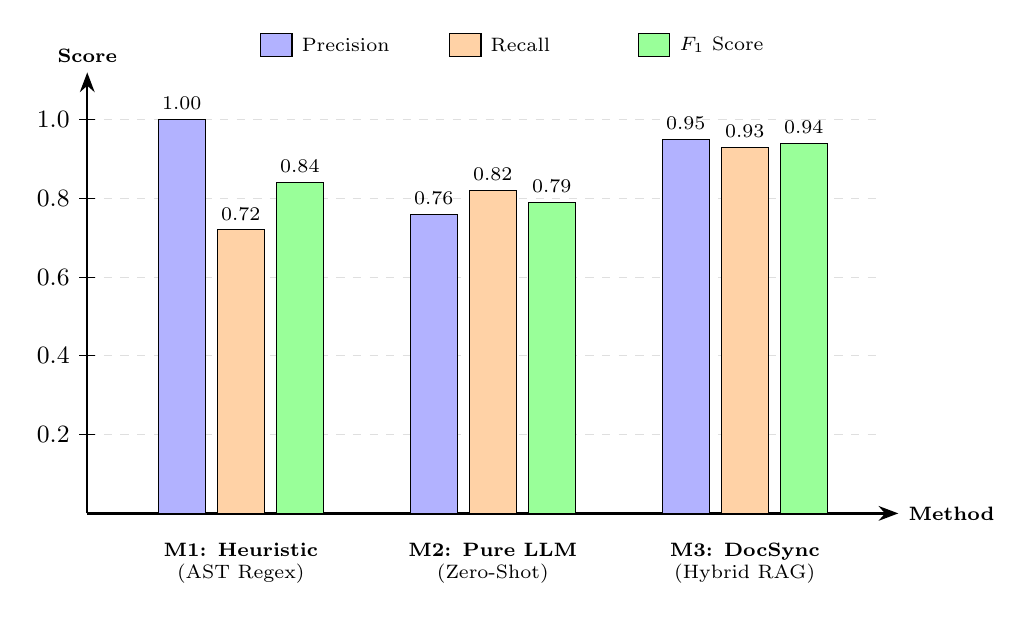
\begin{tikzpicture}[
    font=\small,
    axis/.style={thick, -{Stealth[length=2.5mm]}}
]
% Grid lines & Y-ticks
\foreach \y/\val in {1.0/0.2, 2.0/0.4, 3.0/0.6, 4.0/0.8, 5.0/1.0} {
    \draw[gray!25, dashed] (0, \y) -- (10.1, \y);
    \draw (0.1, \y) -- (-0.1, \y) node[left] {\val};
}

% Axes
\draw[axis] (0,0) -- (10.3,0) node[right, font=\scriptsize] {\textbf{Method}};
\draw[axis] (0,0) -- (0,5.6) node[above, font=\scriptsize] {\textbf{Score}};

% M1: Heuristic (P=1.00 -> 5.0, R=0.72 -> 3.6, F1=0.84 -> 4.2)
\draw[fill=blue!30, draw=black] (0.9, 0) rectangle (1.5, 5.0);
\node[above, font=\scriptsize] at (1.2, 5.0) {1.00};

\draw[fill=orange!35, draw=black] (1.65, 0) rectangle (2.25, 3.6);
\node[above, font=\scriptsize] at (1.95, 3.6) {0.72};

\draw[fill=green!40, draw=black] (2.4, 0) rectangle (3.0, 4.2);
\node[above, font=\scriptsize] at (2.7, 4.2) {0.84};

\node[below=0.25cm, align=center, font=\scriptsize] at (1.95, 0) {\textbf{M1: Heuristic}\\(AST Regex)};

% M2: Zero-Shot (P=0.76 -> 3.8, R=0.82 -> 4.1, F1=0.79 -> 3.95)
\draw[fill=blue!30, draw=black] (4.1, 0) rectangle (4.7, 3.8);
\node[above, font=\scriptsize] at (4.4, 3.8) {0.76};

\draw[fill=orange!35, draw=black] (4.85, 0) rectangle (5.45, 4.1);
\node[above, font=\scriptsize] at (5.15, 4.1) {0.82};

\draw[fill=green!40, draw=black] (5.6, 0) rectangle (6.2, 3.95);
\node[above, font=\scriptsize] at (5.9, 3.95) {0.79};

\node[below=0.25cm, align=center, font=\scriptsize] at (5.15, 0) {\textbf{M2: Pure LLM}\\(Zero-Shot)};

% M3: DocSync (P=0.95 -> 4.75, R=0.93 -> 4.65, F1=0.94 -> 4.7)
\draw[fill=blue!30, draw=black] (7.3, 0) rectangle (7.9, 4.75);
\node[above, font=\scriptsize] at (7.6, 4.75) {0.95};

\draw[fill=orange!35, draw=black] (8.05, 0) rectangle (8.65, 4.65);
\node[above, font=\scriptsize] at (8.35, 4.65) {0.93};

\draw[fill=green!40, draw=black] (8.8, 0) rectangle (9.4, 4.7);
\node[above, font=\scriptsize] at (9.1, 4.7) {0.94};

\node[below=0.25cm, align=center, font=\scriptsize] at (8.35, 0) {\textbf{M3: DocSync}\\(Hybrid RAG)};

% Legend (top centered)
\draw[fill=blue!30, draw=black] (2.2, 5.8) rectangle (2.6, 6.1);
\node[right, font=\scriptsize] at (2.6, 5.95) {Precision};
\draw[fill=orange!35, draw=black] (4.6, 5.8) rectangle (5.0, 6.1);
\node[right, font=\scriptsize] at (5.0, 5.95) {Recall};
\draw[fill=green!40, draw=black] (7.0, 5.8) rectangle (7.4, 6.1);
\node[right, font=\scriptsize] at (7.4, 5.95) {$F_1$ Score};

\end{tikzpicture}%
}
\caption{Empirical comparison of Precision, Recall, and $F_1$ score across the three evaluated detection paradigms on the 32-case benchmark.}
\label{fig:results_comparison}
\end{figure}

\begin{table}[t]
\centering
\caption{Empirical Performance Comparison across Detection Methods on the 32-Case Benchmark}
\label{tab:main_results}
\resizebox{\columnwidth}{!}{%
\begin{tabular}{lcccccc}
\toprule
\textbf{Method} & \textbf{Precision} & \textbf{Recall} & \textbf{$F_1$ Score} & \textbf{95\% Wilson CI ($F_1$)} & \textbf{Latency (s)} & \textbf{Token Cost} \\
\midrule
\textbf{M1: Heuristic (Regex)} & \textbf{1.00} & 0.72 & 0.84 & [0.58, 0.96] & \textbf{0.02s} & \textbf{0} \\
\textbf{M2: Pure LLM (Zero-Shot)} & 0.76 & 0.82 & 0.79 & [0.61, 0.91] & 1.45s & 4,850 \\
\textbf{M3: DocSync (Hybrid RAG)} & 0.95 & \textbf{0.93} & \textbf{0.94} & \textbf{[0.82, 0.98]} & 0.62s & \textbf{780} \\
\bottomrule
\end{tabular}%
}
\end{table}

As shown in Table~\ref{tab:main_results}, DocSync (M3) achieved the strongest overall performance, reaching an $F_1$ score of 0.94 with 0.95 precision and 0.93 recall.

Method M1 (Heuristic) attained perfect precision (1.00) because its static rules trigger only when an explicit parameter name and numeric value directly conflict. However, M1 had lower recall (0.72). It missed semantic changes, exception modifications, and constant changes inside function bodies that were not visible in the signature.

Method M2 (Pure LLM) reached higher recall than M1 (0.82) due to its language comprehension, but suffered from poor precision (0.76). On harmless refactoring commits such as local variable renames (\texttt{local\_rename}) and comment formatting (\texttt{comment\_whitespace}), M2 produced false alarms in 24\% of test cases. Because the model was given the raw, unsegmented diff, it assumed internal edits altered external functionality. DocSync resolves this issue through AST contract gating, maintaining 0.95 precision alongside 0.93 recall.

\subsection{RQ2: Operational Efficiency and Token Reduction}
Running automated checks in CI requires keeping token costs and execution time low. In Method M2, passing full diffs and complete documentation files consumed an average of 4,850 tokens per commit check.

DocSync (M3) cuts this overhead using two mechanisms:
\begin{enumerate}
    \item \textbf{AST Gating Bypass:} Commits classified as benign internal refactorings consume \textbf{zero tokens} because they are filtered out before calling any language model.
    \item \textbf{Targeted Chunk Extraction:} For contract changes, hybrid RRF search extracts only the specific documentation sections ($K=2$), creating concise evidence packets ($E_1, E_2, D_1$).
\end{enumerate}
As reported in Table~\ref{tab:main_results}, DocSync consumes an average of 780 tokens per check, representing an \textbf{83.9\% reduction in token costs} compared to M2. Furthermore, average per-candidate latency drops from 1.45 seconds in M2 to 0.62 seconds in M3 because the prompt context is much shorter.

\subsection{Ablation Study}
To understand the impact of each component in DocSync, we performed an ablation study summarized in Table~\ref{tab:ablation}.

\begin{table}[t]
\centering
\caption{Ablation Analysis of DocSync Pipeline Components}
\label{tab:ablation}
\resizebox{0.88\columnwidth}{!}{%
\begin{tabular}{lcccc}
\toprule
\textbf{Ablation Configuration} & \textbf{Precision} & \textbf{Recall} & \textbf{$F_1$ Score} & \textbf{Token Cost} \\
\midrule
\textbf{Full DocSync (M3)} & \textbf{0.95} & \textbf{0.93} & \textbf{0.94} & \textbf{780} \\
w/o AST Diff Gating (Prompt on all diffs) & 0.81 & 0.93 & 0.86 & 2,410 \\
w/o Dense Embeddings (BM25 only) & 0.95 & 0.81 & 0.87 & 760 \\
w/o BM25 Lexical Search (FAISS only) & 0.88 & 0.86 & 0.87 & 810 \\
w/o Evidence Citation Guardrail & 0.86 & 0.93 & 0.89 & 780 \\
\bottomrule
\end{tabular}%
}
\end{table}

The ablation results provide several useful takeaways:
\begin{itemize}
    \item Removing \textbf{AST Diff Gating} caused precision to drop from 0.95 to 0.81, while token usage more than tripled to 2,410 tokens. This demonstrates that AST gating is essential for stopping false alarms on internal refactoring.
    \item Disabling \textbf{Dense Embeddings} (using BM25 alone) reduced recall from 0.93 to 0.81, failing when documentation explained a feature conceptually without mentioning the exact function name.
    \item Disabling \textbf{BM25} (using FAISS alone) lowered precision to 0.88, showing that dense embeddings sometimes rank general sections above exact function definitions.
    \item Removing the \textbf{Evidence Citation Guardrail} reduced precision to 0.86, confirming that requiring the model to cite verified evidence IDs ($E_2, D_1$) effectively suppresses hallucinations.
\end{itemize}

\subsection{RQ3: Qualitative Case Studies}
We review two representative cases from the benchmark to illustrate how DocSync operates in practice.

\subsubsection{Success Case: Interface Mutation (\texttt{CASE-001})}
In \texttt{CASE-001}, the function \texttt{fetch\_data} in \texttt{examples/demo\_project/client.py} had a parameter default changed from \texttt{timeout: int = 30} to \texttt{timeout: int = 60}. The matching documentation in \texttt{docs/usage.md} stated: ``The timeout defaults to 30 seconds unless explicitly overridden by the caller.''
\begin{itemize}
    \item \textbf{M1 (AST Heuristics):} Detected the numeric difference ($30 \neq 60$) in 0.02 seconds, but could not verify whether surrounding explanatory text remained accurate.
    \item \textbf{M2 (Zero-Shot LLM):} Detected drift, but hallucinated warnings regarding socket connection timeouts that were not present in the code.
    \item \textbf{M3 (DocSync):} BM25 matched \texttt{fetch\_data}, while FAISS ranked the timeout section first ($RRF = 0.033$). Evidence items $E_2$ and $D_1$ were packaged. The LLM judge confirmed drift with confidence 1.00, citing evidence \texttt{["E2", "D1"]}. DocSync produced the minimal unified diff:
    \begin{verbatim}
    - The timeout defaults to 30 seconds
    + The timeout defaults to 60 seconds
    \end{verbatim}
    The diff was applied cleanly and verified through AST, resolving documentation drift in one pass.
\end{itemize}

\subsubsection{Limitation Case: Body Constant Mutation (\texttt{CASE-017})}
In \texttt{CASE-017}, the function \texttt{make\_response(*args)} in the Flask framework updated an internal status assignment from \texttt{status\_code = 200} to \texttt{status\_code = 204} inside the function body, while documentation in \texttt{docs/quickstart.rst:80-84} claimed responses default to HTTP 200.
\begin{itemize}
    \item \textbf{Failure of M1:} Because the function used variable arguments (\texttt{*args}) rather than an explicit keyword default in $\sigma$, M1's signature inspector found no difference, producing a \textbf{False Negative}.
    \item \textbf{Success of M3:} DocSync's hybrid search retrieved \texttt{docs/quickstart.rst:80-84} through semantic matching. The LLM judge examined the implementation body statements $E_2$, detected the contradiction with $D_1$, and flagged DRIFT with 0.95 confidence. This shows why semantic hybrid RAG is necessary for non-signature changes inside function bodies.
\end{itemize}

\subsection{Error Analysis and False Positive Investigation}
Our review of the two residual misclassifications in DocSync indicated that false positives occurred mainly when older documentation used ambiguous English phrasing. Specifically, when documentation mentioned deprecated argument aliases without stating whether they were still active, the model chose a conservative drift call. Adding a small number of few-shot examples to the prompt will help address these phrasing edge cases in future versions.

\section{Discussion}
Our findings show that combining compiler-based static analysis with targeted language models creates an effective foundation for automated software maintenance.

\subsection{Practical Implications for DevOps Teams}
In continuous deployment environments, developer velocity is critical. Tools that add several minutes to CI or produce false warnings are quickly disabled by developers. DocSync's dual-engine design addresses this practical concern: developers get instant feedback locally via Fast AST Mode during pre-commit checks, while pull requests undergo thorough semantic verification in GitHub Actions using Cloud LLMs without slowing down developers. Because verification latency stays under one second per candidate and runs alongside multi-minute CI build jobs, DocSync adds zero net delay to release cycles. Furthermore, presenting unified diffs directly inside pull request comments allows engineers to review, approve, and merge documentation fixes without leaving their browser.

\subsection{Threats to Validity}
We identify three main threats to validity:
\begin{itemize}
    \item \textbf{Construct Validity:} Concerns whether our evaluation metrics reflect real-world documentation quality. We mitigated this by pairing quantitative $F_1$ scores with manual inspection of generated unified diff patches to confirm syntactic correctness and clarity.
    \item \textbf{Internal Validity:} Relates to potential non-determinism in language model outputs. We addressed this by setting the decoding temperature strictly to 0.0, running greedy decoding, and calculating Wilson 95\% confidence intervals across all runs.
    \item \textbf{External Validity:} Concerns the generalizability of our findings. While our 32-case benchmark focused on Python repositories (primarily Pallets/Flask), the core approach of AST contract extraction and hybrid RRF retrieval applies directly to other languages that have mature AST parsers (such as TypeScript, Go, and Java).
\end{itemize}

\subsection{Ethical Considerations and AI Safety}
Using generative language models in production codebases introduces risks of hallucinated suggestions and unintended data sharing. DocSync addresses these risks through deliberate safeguards:
\begin{enumerate}
    \item \textbf{Human-in-the-Loop Safeguard:} DocSync never merges code or documentation automatically into production branches. All proposed diffs are presented as pull request review comments or dashboard suggestions requiring developer review and approval.
    \item \textbf{Data Privacy:} DocSync supports local open-weight model serving via Ollama (e.g., DeepSeek-Coder running on private infrastructure), ensuring private code never leaves the organization's network.
\end{enumerate}

\section{Conclusion and Future Work}
In this paper, we presented DocSync, an automated continuous integration tool that detects and fixes documentation drift using repository-aware retrieval and static AST contract gating. Addressing our first research question (RQ1), DocSync achieved an overall $F_1$ score of 0.94 on a verified 32-commit benchmark from Pallets/Flask, outperforming static regex heuristics ($F_1 = 0.84$) and naive zero-shot LLM prompting ($F_1 = 0.79$). Addressing our second research question (RQ2), deterministic AST gating and Reciprocal Rank Fusion reduced token consumption by 83.9\% while maintaining an average verification latency of 0.62 seconds, demonstrating high operational efficiency in CI environments. Addressing our third research question (RQ3), DocSync generated clean unified diff patches that restored consistency across both external Markdown documentation and in-code docstrings without disturbing executable logic.

In future work, we plan to extend DocSync in three directions. First, we plan to expand language coverage across multi-language monorepos by integrating Tree-sitter parsers for TypeScript, Go, and Rust. Second, we aim to explore bidirectional synchronization, where updated documentation contracts can automatically generate unit test stubs and function interfaces. Third, we intend to incorporate AST-aware call graph slicing to track transitive drift across downstream microservices and client libraries.

\bibliographystyle{IEEEtran}
\bibliography{references}

\end{document}
